

\section{Q3}
\label{part3}
\begin{enumerate}

\item 3.1 Using 20 links that have TimeMaps
\subitem - With 20 or more mementos
\subitem - Have existed 2 years or more (i.e., Memento-Datetime of ``first memento" is April XX, 2013 or older)
\subitem - Note: select from Q1/Q2 links, else choose them by hand

\item 3.2 For each link, create a graph that shows Jaccard Distance, relative to the first memento, through time

\subitem x-axis: continuous time, y-axis: Jaccard Distance relative to the first memento



\end{enumerate}

\subsection{Solution}
\begin{enumerate}

\item I hand picked 20 timemaps from Q2.

\item I wrote a python program to process the timemaps, get the memento URIs, download the boilerpipe representation.

\item Next, I included the code for calculation of jacard distance of all other mementos relative to the first memento.

\item Following are few graphs that shows Jaccard Distance relative to the first memento, through time:


\newpage
\subsubsection{Graphs}
\begin{figure}[ht]    
    \begin{center}
        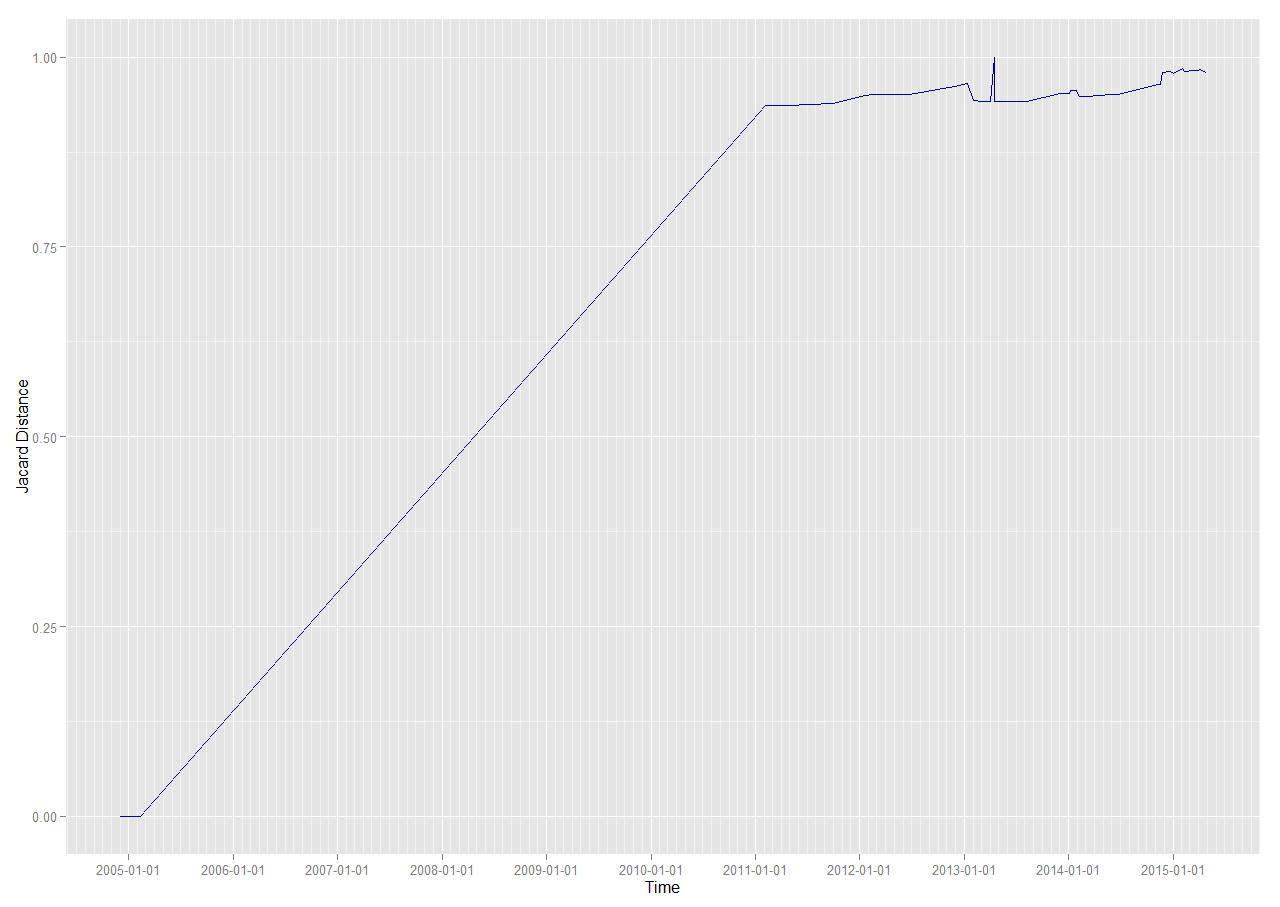
\includegraphics[scale=0.40]{graphs/3_j1.png}
        \caption{Memento 1}
    \end{center}
\end{figure}

\newpage
\begin{figure}[ht]    
    \begin{center}
        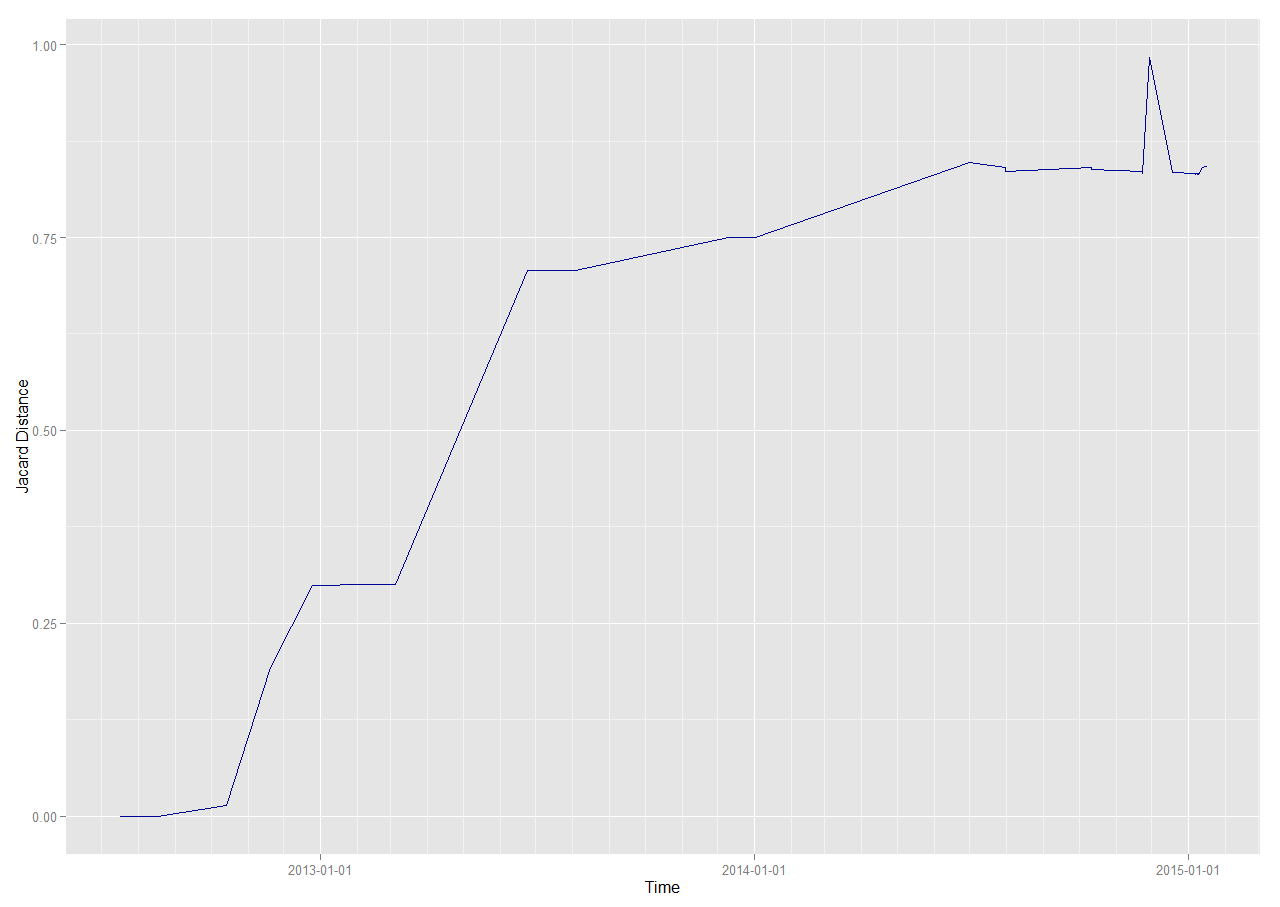
\includegraphics[scale=0.40]{graphs/3_j5.png}
        \caption{Memento 2}
    \end{center}
\end{figure}

\newpage
\begin{figure}[ht]    
    \begin{center}
        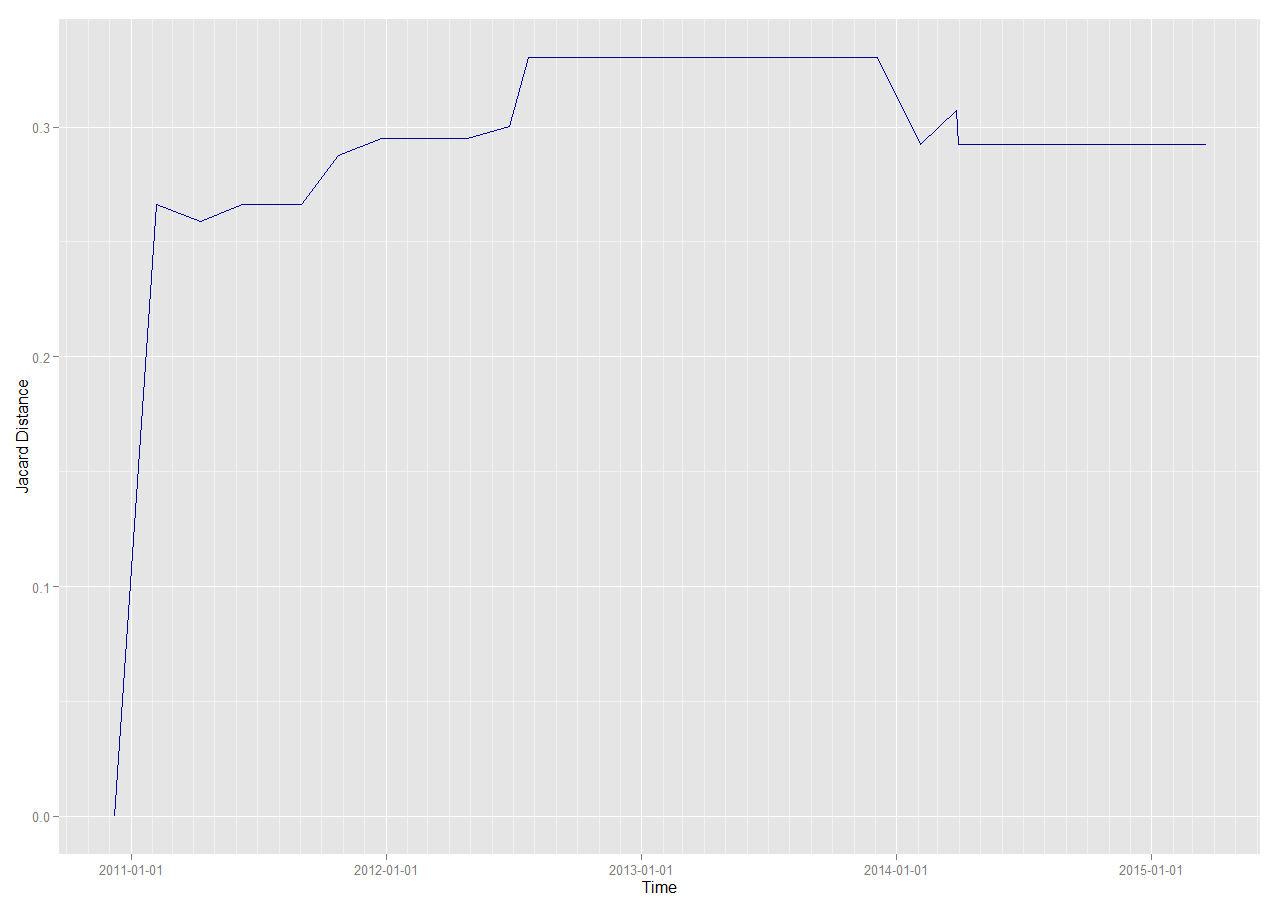
\includegraphics[scale=0.40]{graphs/3_j6.png}
        \caption{Memento 3}
    \end{center}
\end{figure}

\newpage
\begin{figure}[ht]    
    \begin{center}
        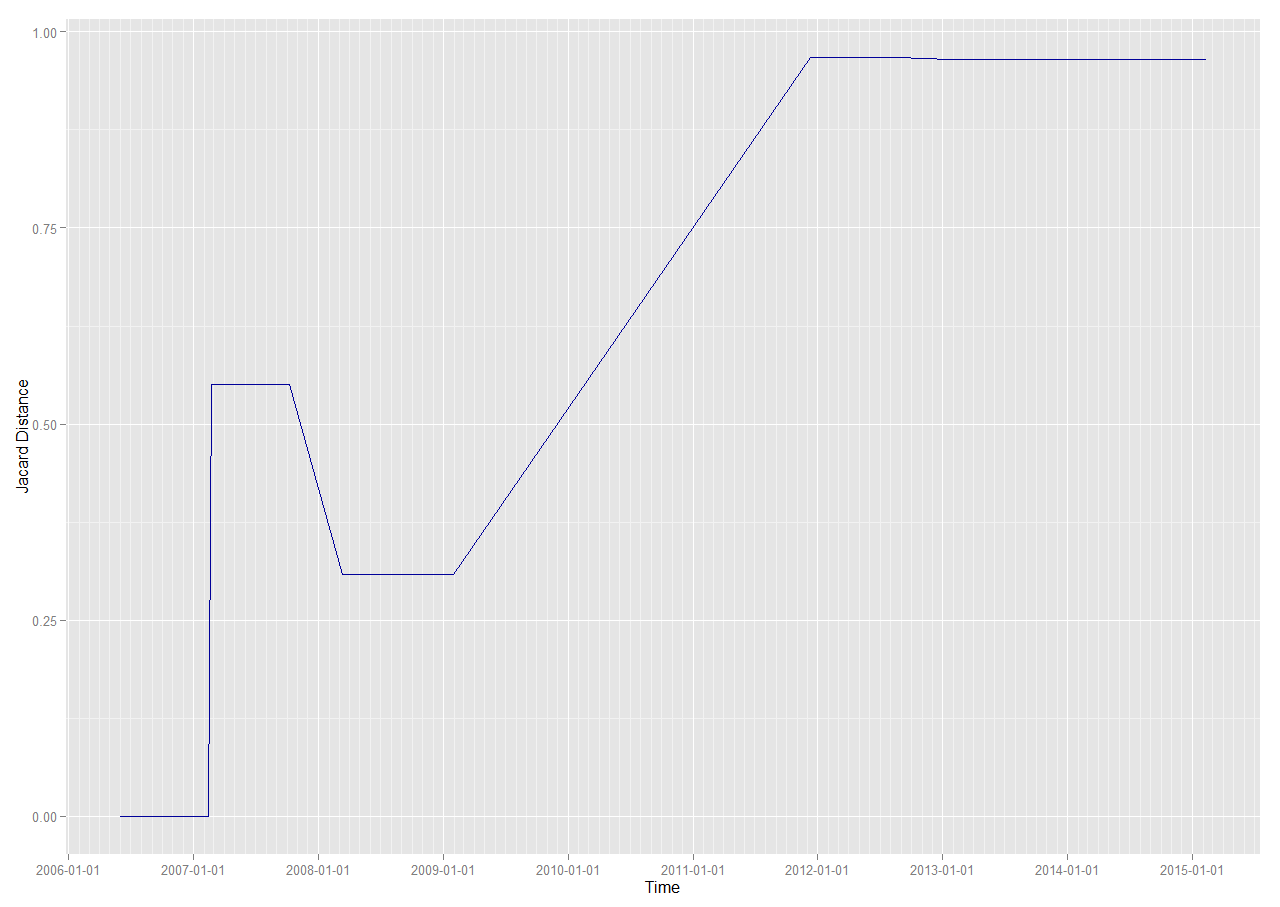
\includegraphics[scale=0.40]{graphs/3_j7.png}
        \caption{Memento 4}
    \end{center}
\end{figure}



\newpage
\subsection{Code Listing}
\subsubsection{Python program to using boilerpipe library to extract just the text from HTML documents of the mementos for the selected 20 timemaps}
\lstinputlisting[language=Python,breaklines = true,frame=single, label=lst:q1-1,captionpos=b,numbers=left,showspaces=false,showstringspaces=false,basicstyle=\footnotesize]{src/3.fetchBoilerpipeForMementos.py}
\newpage

\subsubsection{R code to plot CDF}
\lstinputlisting[language=Python,breaklines = true,frame=single, label=lst:q1-1,captionpos=b,numbers=left,showspaces=false,showstringspaces=false,basicstyle=\footnotesize]{src/3.r}

\end{enumerate}

